\documentclass[a0,portrait,final]{a0poster}

\usepackage{calc}
\usepackage{epsfig}
\usepackage{xspace}
\usepackage{amsmath}
\usepackage{wrapfig}
\usepackage{multirow}
\usepackage{rotating}
\usepackage{arydshln}
\usepackage{booktabs}
\usepackage{multicol}
\usepackage{enumitem}
\usepackage{inconsolata}
\usepackage[english]{babel}
\usepackage{pstricks,pst-grad}
\usepackage{hyperref}
\usepackage{listings}
\usepackage{color}

\newcommand{\tail}[1]{$Q_{tail}${}}
\newcommand{\head}[1]{$Q_{head}${}}
\newcommand{\stail}[1]{$S_{tail}${}}
\newcommand{\shead}[1]{$S_{head}${}}
\newcommand{\etail}[1]{$E_{tail}${}}
\newcommand{\ehead}[1]{$E_{head}${}}


\newrgbcolor{bluisti}{0.02 0.23 0.38}% #073B62 R7 G59 B98
\newrgbcolor{arancioneisti}{0.98 0.44 0.08}% #FC7216 R252 G114 B22
%\newrgbcolor{orangered}{1 0.14 0.00}%orangered rgb(100%, 14%, 0%
%\newrgbcolor{rosso}{0.80 0.00 0.00}%
%\newrgbcolor{yahoo}{0.40 0.00 0.60}%concord grape rgb(40%, 0%, 60%)
%\newrgbcolor{verde}{0.0 0.702 0.0}

\setlength{\columnsep}{1in}
\setlength{\parindent}{0.0cm}

\newcommand{\pbox}[3]{
	\begin{center}
	\psshadowbox[linewidth=2mm,framearc=0.1,framesep=1em,shadowsize=4mm,shadowcolor=lightgray,linecolor=#2]{
		\begin{minipage}[t][][t]{#1}{
			#3 %text
		}\end{minipage}
	}
	\end{center}
}

\newcommand{\dexter}[1]{{\sf Dexter}\xspace}

\newlength\ptitlespace
\setlength\ptitlespace{2.6cm}

\newcommand{\ptitle}[1]{
	\vspace{\ptitlespace}
	\pbox{0.92\columnwidth}{arancioneisti}{
		\begin{center}
		\textsc{\LARGE\bluisti{#1}} %text
		\end{center}
	}
	\vspace{0.5\ptitlespace}
}

\newcommand{\btitle}[1]{\begin{center} \Large{\textsc{#1}} \end{center} \vspace{1.5cm}}
	
\begin{document}
	\newlength\logosize
	\setlength\logosize{8cm}
	\pbox{0.96\textwidth}{arancioneisti}{
	\centering
	\begin{tabular}{ccc}
		\begin{minipage}[c]{\logosize}
		\centering
			
\includegraphics[width=5cm]{img/ucl.eps}
		\end{minipage}
	&
		\begin{minipage}[c]{0.98\textwidth-2\logosize}
		\centering\textsc{}
		\Huge \textsc{Bringing the Head Closer to the Tail\\ with Entity Linking}\\[8mm]
	\Large{Manisha Verma$^{1}$, Diego Ceccarelli$^{2,3}$}\\
	\Large{$^1$ UCL Department Of Computer Science}
	\Large{$^2$ ISTI-CNR, Pisa, Italy}\hspace{2cm}\Large{$^3$ IMT Lucca}\\
	
		\end{minipage}
	& 

	\begin{minipage}[c]{\logosize}
	\centering
	
	\end{minipage}
		\begin{minipage}[c]{\logosize}
		\centering
		
\includegraphics[width=9cm]{img/logohpc.eps}
		\includegraphics[width=5cm]{img/logoisti.eps}
		\end{minipage}
	\end{tabular}
	}


\vfill
\large


\begin{multicols}{2}
	
	With the creation and rapid development of knowledge bases, it has become easier
	 to understand the \textbf{underlying semantics of unstructured text} (short or long) on the web.  
	 In this work we especially look at the impact of entity linking on search logs. 
	 Search queries follow a \emph{Zipfian} distribution wherein other than few popular queries 
	 (\emph{head queries}), a significant percentage of queries (\emph{tail queries}) occur rarely. 
	 Given a search log, there is sufficient data to analyze head queries but insufficient 
	 data (low frequency, limited clicks) to draw any conclusions about tail queries. 
	%Search queries are primary means of finding information. While a handful of 
	 %queries account for majority of search volume, a large number of queries 
	 %occur infrequently. The individual frequency and sparsity of related statistics makes 
	 %it difficult to draw any conclusions about such rare queries.
	 %renders it difficult to draw any conclusions about the nature of the query. 
	 In this work we focus on quantifying the extent of \textbf{overlap between long tail
	 	 and head queries} by means of entity linking. We specifically analyze the 
	 frequency distribution of entities in head and tail queries. 
	 %We also analyze the ratio of popular entities to rare entities in tail queries. 
	
	 
	  \vspace{10mm}
	  \begin{center}
	  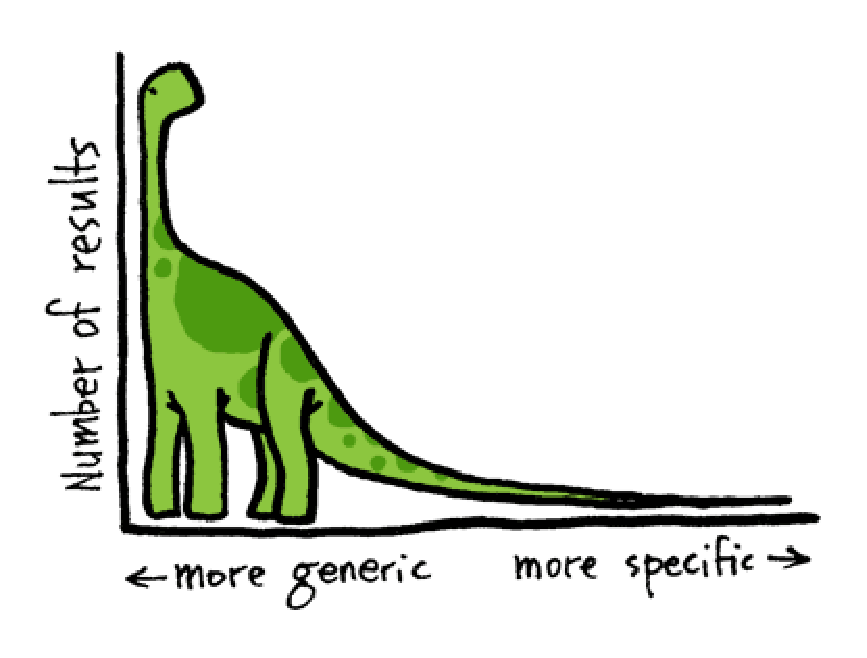
\includegraphics[width=0.9\columnwidth]{img/long-tail.eps}
	  \end{center}
	  
 \ptitle{Research Questions}
  
	  we are interested in studying the 
	  relationship between the head and the tail queries through the entities they contain. 
	  Our primary research questions are:
	  \begin{itemize}
		\LARGE 
	  	\item Are tail queries a different means to inquire about entities mentioned in the head queries? 
	  	\item Can we find tail queries about entities that are not searched in the head (we will call them \emph{tail entities})?
	  	\item Can we find a relationship between \emph{ tail entities} and \emph{head entities}?  
	  \end{itemize}
	 
\ptitle{AOL Query Log}

We perform our analysis on the AOL query log, since it is publicly available\footnote{\url{http://www.gregsadetsky.com/aol-data/}}. AOL log consists of approximately 20 million queries submitted by $650,000$ users from March to May 2006. Queries are normalized (text lowercased, non ascii characters removed) and there are in total $10,154,742$ distinct queries. 
We extract 2 distinct sets from these queries: 
\begin{description}
	\item{\tail{}} The set of queries in the long tail, i.e. queries that appear in the log with a frequency \emph{lower than or equal} to $2$. The set contains $7,746,607$ distinct queries, i.e. $76\%$ of distinct queries, but it is $26\%$ of the total volume of the queries.
	\item{\head{}} The set of queries in the head. It contains queries that appear with a frequency \emph{greater than} $99$. The set contains $19,953$ distinct queries, i.e. $0.002\%$ if we look at the distinct queries, but still these queries represent $26\%$ of total query volume.% if we consider the frequencies of the queries.
\end{description}
Although, the two sets differ in number of queries ($\sim19$K versus $\sim7$M), they cover the same fraction of total queries issued to the search engine. All our analysis are performed on these two sets.



\ptitle{Entity Linking Problem}

The entity linking task aims at identifying, given a plain document, the small fragments of text (interchangeably called \emph{mentions} or \emph{spots}) referring to any \emph{named entity} that is listed in a given knowledge base, e.g. Wikipedia. The ambiguity of natural language makes it a non trivial task. The same entity can be in fact mentioned with different text fragments, e.g., ``President Kennedy'' or ``John F. Kennedy''. On the other hand, the same mention may refer to different entities, e.g., ``Michael Collins'' may refer to either the well known astronaut, or to the Irish leader and president of the Irish provisional government in 1922.

\vspace{5mm}
\begin{center}
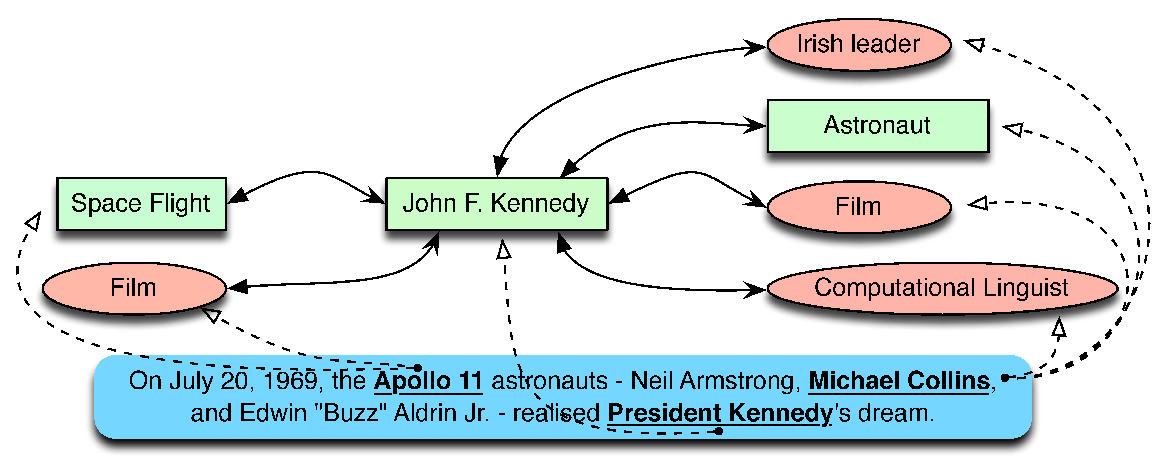
\includegraphics[width=0.92\columnwidth]{img/annotation-example.eps}
\end{center}

The annotation is usually organized in three subtasks:
\begin{enumerate}
	\item \textbf{Spotting}: discover the fragments that could refer to an entity. A set of candidate mentions is detected, and for each mention a list of candidate entities is produces;
	\item \textbf{Disambiguation}: for each spot associated with more than one candidate, a single entity is selected to be linked to the spot;
	\item \textbf{Ranking}: the list of entites detected is ranked according to some policy, e.g. annotation confidence. 
\end{enumerate}

Our entity linker Dexter (\url{dxtr.it}) identifies 
at least one spot in $13,977$ ($70\%$) and $4,901,987$ ($63\%$) \head{} and \tail{} 
respectively.

\ptitle{Analysis}


\begin{tabular}{lc|lc|lc|lc}
\toprule
\multicolumn{4}{c}{\head{}} & \multicolumn{4}{c}{\tail{}}\\
\multicolumn{2}{c}{\shead{}} & \multicolumn{2}{c}{\ehead{}} & \multicolumn{2}{c}{\stail{}} & \multicolumn{2}{c}{\etail{}}\\
\midrule
google         & 342,602  &  Google  		   & 349,337  &  florida 	 &	47,718	&	Florida 		& 49,366 \\
myspace        & 194,093  &  Yahoo\!  		   & 299,718  &  texas  	 &	 37,388  &   Texas   		& 37,526 \\
yahoo          & 142,361  &  Myspace 		   & 289,353  &  ohio    	 &	31,861   &   Ohio    		& 31,905 \\			
ebay           & 142,257  &   EBay   		   & 187,633  &  edu     	 &	26,641   &   New\_York        & 28,396 \\
yahoo.com      & 104,696  &  MapQuest          & 135,179  &  state   	 &	26,066   &   .edu    		& 26,642 \\
mapquest       & 88,617   &  Google\_Search     & 98,112   &  california  &   25,233  &   U.S.\_state      & 26,392 \\
google com     & 85,670   &  Hotmail           & 53,925   &  new york    &   24,865  &   California      & 25,859 \\
my space       & 48,401   &	  Bank\_of\_America  & 46,922   &  hotel   	 &	20,018   &   Real\_estate     & 25,232 \\
www.yahoo.com  & 44,198   &  Craigslist        & 45,586   &  real estate &   19,702  &   Myspace 		& 24,998 \\
internet       & 39,865   &  Ask.com           & 39,873   &  myspace 	 &	18,533   &   Floruit 		& 24,207 \\
ebay com       & 30,652   &  Internet          & 39,865   &  restaurant  &  17,065   &   Restaurant      & 21,996 \\
hotmail.com    & 28,492   &  Pornography       & 35,089   &  michigan    &   15,635  &   Hotel   		& 20,289 \\
map quest      & 27,949   &  Tattoo            & 33,113   &  new jersey  &   14,813  &   Nudity  		& 18,245 \\
craigslist     & 27,222   &  American\_Idol     & 28,890   &  georgia 	 &	14,525   &   United\_States   & 16,680 \\
american idol  & 23,665   &  Yahoo!\_Mail       & 28,238   &  black   	 &	13,921   &   Michigan        & 15,763 \\
\bottomrule
\end{tabular}




% \ptitle{Motivations}
% Several entity linking algorithms were recently proposed for annotating documents with entities. Performing a fair comparison among these techniques is very hard. To the best of our knowledge, only a few authors released the source code of their algorithms or provide
% a REST API for annotating documents using their method. As a result, evaluating today the performance of a method on a single subtask, comparing different techniques or mixing different strategies together is difficult.
%
% \vspace{4mm}
% \textbf{We strongly believe that it is important to share a unique framework where each subtask is well separated and easy to isolate in order to study its performance, perform fair comparisons and improve the state of the art.}
%
%
% \ptitle{Dexter Framework}
%
% In this work we present a new open source framework, called Dexter, that implements some popular algorithms and provides several tools useful to develop an entity linking technique.
%
% % \vspace{10mm}
% % \begin{center}
% % \includegraphics[width=0.20\columnwidth]{img/dexter-logo.eps}
% % \end{center}
%
% \vspace{10mm}
% \begin{center}
% \includegraphics[width=0.80\columnwidth]{img/screenshot.eps}
% \end{center}
%
% \ptitle{Dexter Architecture}
%
% Dexter is developed in Java and is organized in several Maven modules.
%
% \vspace{10mm}
% \begin{center}
% \includegraphics[width=0.8\columnwidth]{./img/dexter-architecture.eps}
% \end{center}
%
% \ptitle{Plug and Play}
%
% \lstset{language=Java,
%  		   basicstyle=\fontsize{24}{26}\ttfamily,
%            keywordstyle=\color{blue}\ttfamily,
%            stringstyle=\color{red}\ttfamily,
%            commentstyle=\color{green}\ttfamily}
% \begin{lstlisting}
% public class TopScoreEntityDisambiguator implements Disambiguator {
%         @Override
%         public EntityMatchList disambiguate(SpotMatchList sml) {
%                 EntityMatchList eml = new EntityMatchList();
%                 for (SpotMatch match : sml){
%                         EntityMatchList list = match.getEntities();
%                         if (! list.isEmpty()){
%                                 list.sort();
%                                 eml.add(list.get(0));
%                         }
%                 }
%                 return eml;
%         }
% }
% \end{lstlisting}
%
% \ptitle{Conclusion and Future Work}
%
% \begin{itemize}
% \item We implemented two state-of-the-art methods in Dexter: TAGME and Wikiminer. We plan to implement several other state of the art approaches in order to show their performance and efficiency on a wide range of datasets;
% \item We plan to investigate the performance of the entity linking methods on different evaluation datasets. We have recently released
% \textbf{Elianto}  a web-deployed tool that allows to crowdsource the creation of manually annotated datasets;
% \item We plan to support different Wikipedia languages (actually only English is supported);
% \item We intend to improve the performance of the annotator, in terms of result's quality, response time and resource usage.
% \end{itemize}
%
% \ptitle{Fork me on Github!}
%
% The code is available on Github at the following address:
% \begin{itemize}
% 	\item \url{https://github.com/diegoceccarelli/dexter}
% \end{itemize}
%
% A demo webapp and some other useful informations can be found here:
% \begin{itemize}
% 	\item \url{http://www.dxtr.it}
% \end{itemize}

\end{multicols}
\vfill
\centering
\begin{minipage}[c]{\textwidth}
\rule{\textwidth}{1pt}
\textit{ESAIR '14  -- 7$^\textit{th}$ International Workshop on Exploiting Semantic Annotations in Information Retrieval. November 7, 2014. Shanghai, China.}
%\textit{ESAIR '14  -- The 23\emph{rd} ACM Conference on Information \& Knowledge Management. November 3-7, 2014. Shanghai, China}
\end{minipage}

\end{document}